\documentclass{article}

\usepackage{microtype}
\usepackage{graphicx}
\usepackage{subfigure}
\usepackage{booktabs}
\usepackage{hyperref}

\newcommand{\theHalgorithm}{\arabic{algorithm}}

\usepackage[accepted]{icml2021}

\begin{document}

\twocolumn[
\icmltitle{House Price Prediction}

\begin{icmlauthorlist}
\icmlauthor{Jeremy Guan}{}
\icmlauthor{Cheng-Cheng Liu}{}
\icmlauthor{Xudong Zhang}{}
\icmlauthor{Yixiao Li}{}
\end{icmlauthorlist}

\vskip 0.3in
]

\section{Results}

We evaluated multiple machine learning models for house price prediction using the Kaggle House Prices dataset, 
which contains 1460 training examples and 79 explanatory variables describing residential homes in Ames, Iowa. All models were 
trained using 5-fold cross-validation and evaluated using Root Mean Squared Error (RMSE) in log-space.

\subsection{Model RMSE Comparison}

Figure~\ref{fig:modelcomparison} summarizes the final RMSE performance across all implemented models.

\begin{figure}[h]
\centering
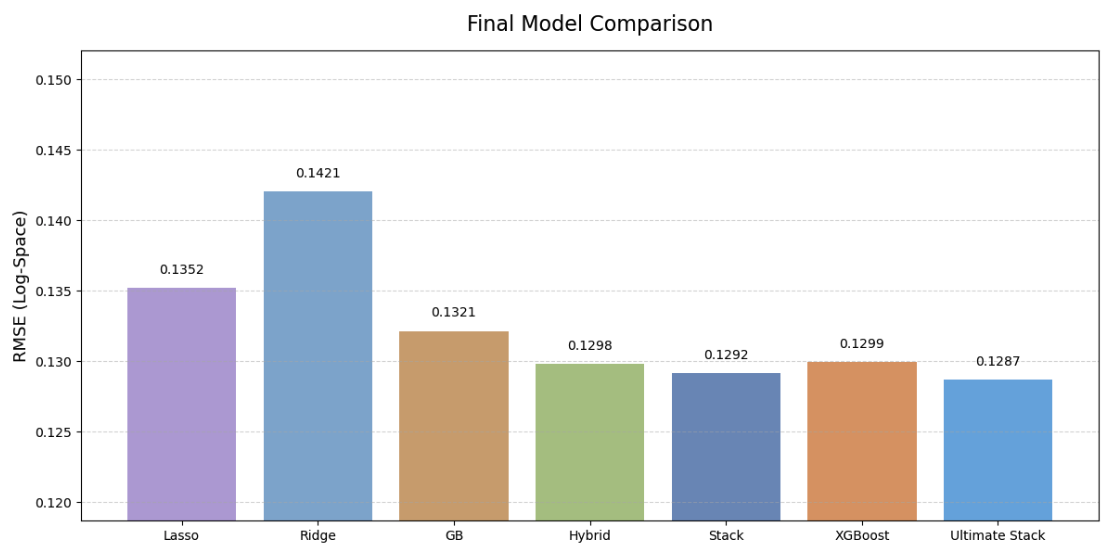
\includegraphics[width=1\linewidth]{finalGraphComparison.png}
\caption{Final RMSE comparison across all models. Lower RMSE indicates better performance.}
\label{fig:modelcomparison}
\end{figure}

Among the linear models, Lasso Regression achieved slightly lower RMSE than Ridge Regression because L1 regularization performs 
implicit feature selection by shrinking less important coefficients to zero.

Nonlinear models performed substantially better overall. Gradient Boosting significantly outperformed the linear approaches, 
suggesting that housing prices contain strong nonlinear relationships that simple linear models cannot fully capture.

The Hybrid and Stacking models provided additional improvements beyond standalone Gradient Boosting. XGBoost achieved performance 
comparable to Gradient Boosting, while the Ultimate Stacking model achieved the best overall RMSE of 0.1287 by combining predictions 
from Lasso Regression, Gradient Boosting, and XGBoost.

Although the improvements from ensemble methods were relatively modest, the results suggest that combining more diverse 
nonlinear learners provides additional complementary predictive information.

\subsection{Ultimate Stack Model}

\begin{figure}[h]
\centering
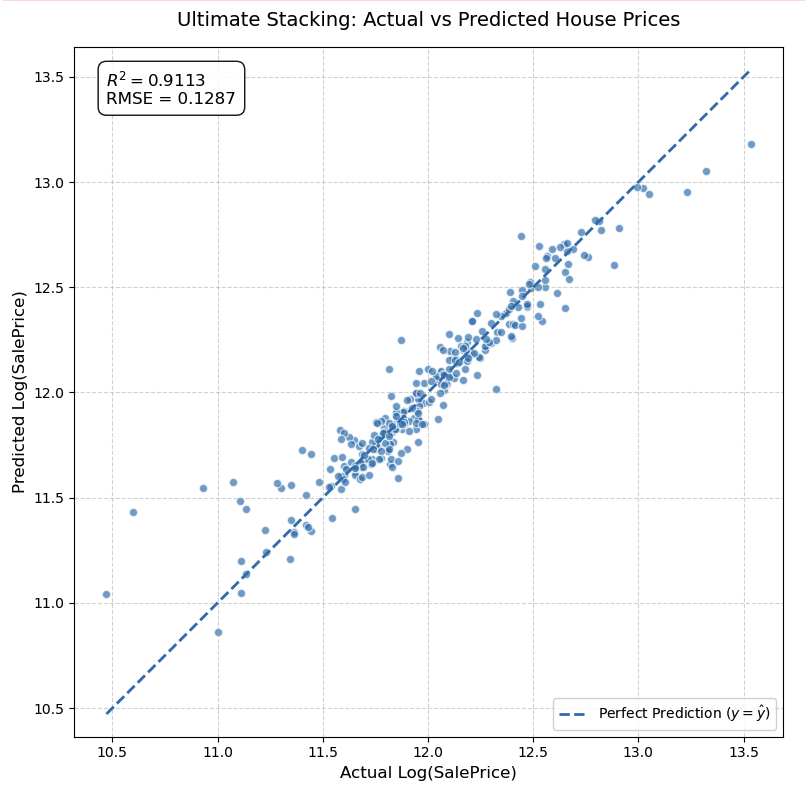
\includegraphics[width=1\linewidth]{ultimateStack.png}
\caption{Ultimate Stacking predictions versus actual house prices in log-space. The dashed diagonal line represents 
perfect predictions.}
\label{fig:stackingpred}
\end{figure}

Since the Ultimate Stacking model achieved the lowest overall RMSE among all evaluated approaches, 
we focus our detailed prediction analysis on this model. Presenting only the best-performing model provides a clearer 
visualization of overall prediction quality and remaining errors without introducing redundant plots for weaker models.

Figure~\ref{fig:stackingpred} shows the prediction quality of the Ultimate Stacking model on the final test set. 
Most predictions lie close to the diagonal reference line, indicating a strong relationship between predicted and actual 
housing prices. The model achieved an $R^2$ score of 0.9113, indicating that the ensemble model successfully explained 
most of the variance in house prices.

Although most homes were predicted accurately, several outliers remain visible, particularly among extremely expensive homes. 
These prediction errors likely occur because luxury properties and rare neighborhood characteristics are underrepresented 
in the training data. In addition, some housing attributes may interact non-linearly in ways that are difficult for 
tabular features to fully capture. Overall, the prediction results demonstrate that ensemble methods generalized 
effectively and produced highly accurate predictions across a wide range of housing prices.

\subsection{Ultimate Stack Weights}

\begin{figure}[t]
\centering
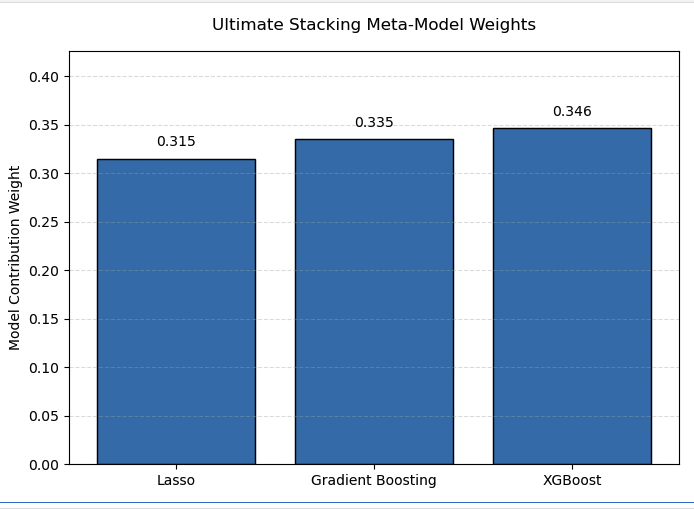
\includegraphics[width=0.9\linewidth]{stacking_weights.png}
\caption{Meta-model weights learned by the Ultimate Stacking ensemble. Larger weights indicate stronger contribution to the final prediction.}
\label{fig:stackweights}
\end{figure}

Figure~\ref{fig:stackweights} shows the contribution weights learned by the stacking meta-model. XGBoost and Gradient Boosting 
received the largest weights, indicating that nonlinear tree-based learners contributed most strongly to the final predictions. 
Lasso Regression still provided complementary predictive information, suggesting that combining both linear and nonlinear modeling 
approaches improved overall ensemble performance.

\subsection{Residual Analysis}

\begin{figure}[h]
\centering
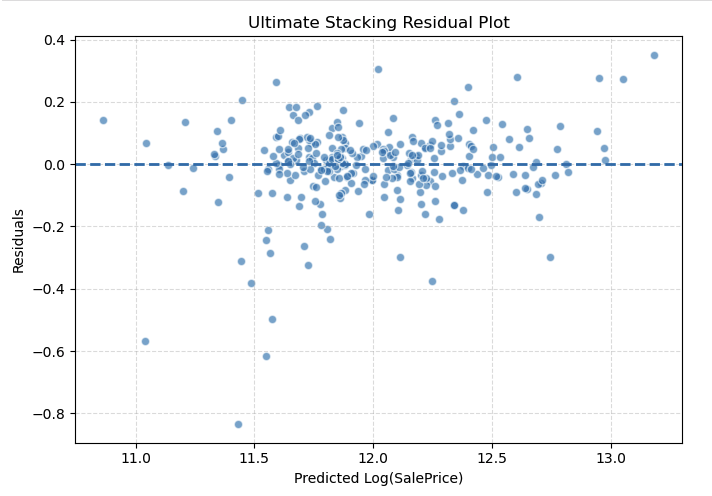
\includegraphics[width=1\linewidth]{residual_plot.png}
\caption{Residual plot of the Ultimate Stacking model. Residuals remain centered near zero, indicating limited systematic prediction bias.}
\label{fig:residuals}
\end{figure}

Figure~\ref{fig:residuals} shows the residual distribution of the Ultimate Stacking model. Most residuals remain concentrated around zero, indicating that the model does not exhibit strong systematic prediction bias. Larger residual variance appears primarily among expensive homes, suggesting that luxury properties remain more difficult to predict accurately due to rare or highly nonlinear housing characteristics.
Manual inspection of several high-error predictions revealed that many poorly predicted homes contained uncommon feature combinations, including unusually large living areas, premium neighborhoods, and extensive renovations. These rare housing configurations were underrepresented in the training data, making accurate generalization more challenging for the ensemble model.
\subsection{Discussion}

Overall, the experimental results demonstrate that ensemble learning provides the strongest predictive performance for tabular housing datasets. 
While regularized linear models improved substantially over the baseline regression model, nonlinear boosting approaches captured more complex 
relationships between housing attributes and sale prices. Combining both linear and nonlinear learners within the Ultimate Stacking framework 
produced the most accurate and robust predictions across the full range of housing prices.

The results also highlight the importance of preprocessing and feature engineering. Missing-value handling, log transformation, one-hot encoding, 
and feature scaling all contributed to improving model stability and reducing overfitting. These findings suggest that both data preprocessing 
and ensemble learning are critical for achieving strong performance on structured real-world machine learning problems.

% =====================================================
% Bibliography
% =====================================================

\bibliography{references}
\bibliographystyle{icml2021}

\end{document}